\documentclass[a4paper,11pt]{report}
\usepackage[T1]{fontenc}
\usepackage[utf8]{inputenc}
\usepackage[francais]{babel}
\usepackage{graphicx}
\usepackage{verbatim}
\usepackage{moreverb}
\usepackage{hyperref}
\usepackage{tikz}
\usepackage{amssymb}
\usepackage{amsmath}
\usepackage{fullpage}
\usepackage{xcolor}
\usepackage{listings}
\usepackage{algorithm}
\usepackage{algpseudocode}
\usepackage{latexsym}
\usepackage{ucs}
\usepackage{pdfpages}
\usetikzlibrary{arrows,positioning,automata,shadows,matrix,calc}

\usepackage{amsthm}
\newtheorem{corollary}{Corollaire}[section]
\newtheorem{definition}{Définition}[section]
\newtheorem{example}{Exemple}[section]
\newtheorem{lemma}{Lemme}[section]
\newtheorem{proposition}{Proposition}[section]
\newtheorem{remark}{Remarque}[section]
\newtheorem{theorem}{Théorème}[section]

\renewcommand{\algorithmicrequire}{\textbf{Input:}}
\renewcommand{\algorithmicensure}{\textbf{Output:}}

\newcommand{\reporttitle}{SIMULATION DE PARTICULES SUR ARCHITECTURES PARALLÈLES}     % Titre
\newcommand{\reportauthor}{- Henri Frank \textbf{ANABA}\\ - Olivier \textbf{Constans}}% Auteur
\newcommand{\reportsubject}{Programmation Multicoeur} % Sujet

\hypersetup{
    pdftitle={\reporttitle},%
    pdfauthor={\reportauthor},%
    pdfsubject={\reportsubject},%
    pdfkeywords={rapport} {vos} {mots} {clés}
}

\lstdefinestyle{CStyle}{ 
  language=C,
  basicstyle=\small\sffamily,
  numberstyle=\tiny,
  numbersep=3pt,
  frame=single,
  columns=fullflexible,
  backgroundcolor=\color{yellow!30},
  commentstyle=\itshape\color{purple!40!black},
  linewidth=0.9\linewidth, 
  xleftmargin=0.1\linewidth }



\begin{document}

\newcommand{\Aut}{\mathcal{A}}
\newcommand{\N}{\mathbb{N}}
\newcommand{\R}{\mathcal{R}}
\newcommand{\T}{\mathcal{T}}
\newcommand{\F}{\mathcal{F}}
\newcommand{\HRule}{\rule{\linewidth}{0.5mm}}

%\begin{titlingpage}
\begin{center}

\begin{minipage}[t]{0.48\textwidth}
  \begin{flushleft}
    
\includegraphics [width=50mm]{images/index.png} \\[0.5cm]
  \end{flushleft}
\end{minipage}
\begin{minipage}[t]{0.48\textwidth}
  \begin{flushright}
  %  \includegraphics [width=30mm]{images/logo-societe.jpg} \\[0.5cm]
   % \textsc{\LARGE Entreprise}
  \end{flushright}
\end{minipage} \\[1.5cm]

\textsc{\Large \reportsubject}\\[0.5cm]
\HRule \\[0.4cm]
{\huge \bfseries \reporttitle}\\[0.4cm]
\HRule \\[1.5cm]

\vfill

\begin{minipage}[t]{0.6\textwidth}
  \begin{flushleft} \large
    \emph{Auteurs :}\\ 
    \reportauthor
  \end{flushleft}
\end{minipage}

\hfill
\vfill
\vfill
\vfill

\begin{minipage}[t]{0.6\textwidth}
  \begin{flushright} \large
    \emph{Responsable :} \\
    M.~R \textsc{NAMYST}\\
  \end{flushright}
\end{minipage}

\vfill

{\large \today}

\end{center}

%\end{titlingpage}

\newpage

%\frontmatter
\begingroup
%\setlength{\beforechapskip}{0pt} % or any other dimension
\tableofcontents
\endgroup

%\mainmatter


\chapter{Présentation du sujet}

\paragraph{}
Dans le cadre du module d'enseignement de programmation parallèle, nous devons réaliser un projet. Ce projet consiste en la conception d'une application de simulation de particules dans un domaine en trois dimensions. Pour ce faire, il a été mis à notre disposition un rendu OpenGL des particules ainsi que son code et une version séquentielle du code. Le rendu permet de visualiser la simulation en temps réel. Le but étant que nous nous concentrions uniquement sur l'accélération des calculs en parallèle.
\paragraph{}
Ce rapport présente le travail réalisé par le binôme constitué de Henri Frank \textbf{ANABA} et d'Olivier \textbf{CONSTANS}.Il est en effet le compte-rendu de la réalisation  des deux parties  du projet : la partie \textbf{OpenMP} et la partie  \textbf{OpenCL}


\chapter{Traitement du sujet}
\section{Parallélisation avec \textbf{OpenMP}}

\subsection{Parallélisation des boucles}

\paragraph{}
La réalisation de la version de base consistait juste en une parallélisation des boucles de la version séquentielle. Pour ce, nous avons choisi d'utiliser la directive OpenMP pour la parallélisation des boucles \textbf{for} \#pragma omp for. 

\paragraph{}
Pour chaque fonction appelée par la fonction principale de simulation, nous avons optimisé le calcul des boucles for.Dans la fonction, \textbf{omp\_update\_vbo}, parallélisation de la boucle de mise à jour des vitesses des atomes :
\newline
\begin{lstlisting}[style=CStyle]
static void omp_update_vbo (sotl_device_t *dev)
{
  sotl_atom_set_t *set = &dev->atom_set;
  sotl_domain_t *domain = &dev->domain;

   #pragma omp for
  for (unsigned n = 0; n < set->natoms; n++) {
    ...
  }
}
\end{lstlisting}

\paragraph{}
Dans la fonction, \textbf{omp\_move}, parallélisation de la boucle de mise à jour des vitesses de chaque atome :
\newline
\begin{lstlisting}[style=CStyle]
static void omp_move (sotl_device_t *dev)
{
  sotl_atom_set_t *set = &dev->atom_set;

  #pragma omp for
  for (unsigned n = 0; n < set->natoms; n++) {
    set->pos.x[n] += set->speed.dx[n];
    set->pos.y[n] += set->speed.dy[n];
    set->pos.z[n] += set->speed.dz[n];
  }
}
\end{lstlisting}
\paragraph{}
Dans la fonction, \textbf{omp\_ gravity}, parallélisation de l'application de la gravité aux vitesses des atoms:
\newline
\begin{lstlisting}[style=CStyle]
static void omp_gravity (sotl_device_t *dev)
{
  sotl_atom_set_t *set = &dev->atom_set;
  const calc_t g = 0.005;
  #pragma omp for
   for (unsigned current = 0; current < set->natoms; current++) {
	set->speed.dy[current] = set->speed.dy[current]-g;
  }
}
\end{lstlisting}
%%%%%%%%%%%%%%%%%%%%%%%%%%%%%%%%%

\paragraph{}
Dans la fonction \textbf{omp\_bounce}, parallélisation de la boucle de calcul.
\newline
\begin{lstlisting}[style=CStyle]
static void omp_bounce (sotl_device_t *dev)
{
  sotl_atom_set_t *set = &dev->atom_set;
  sotl_domain_t *domain = &dev->domain;
    #pragma omp for
     for (unsigned current = 0; current < set->natoms; current++) {
	...
     }
}
\end{lstlisting}
%%%%%%%%%%%%%%%%%%%%%%%%%%%%%

\paragraph{}
Dans la fonction \textbf{tri}, parallélisation des boucles de permutation des atomes lors du tri:
\newline
\begin{lstlisting}[style=CStyle]
void tri(sotl_atom_set_t * set){

  int paire = (set->natoms%2==0)?1:0;
  int impaire = (set->natoms%2==0)?0:1;
  for(unsigned i=0; i<set->natoms; i++){
    if(i%2==0){
      #pragma omp parallel
      #pragma omp for schedule(runtime)
      for(unsigned j =0; j<set->natoms-impaire;j+=2){
	if(set->pos.z[j]<set->pos.z[j+1]){
	 echange(set,j,j+1);
	}
      }
    }else{

      #pragma omp parallel
      #pragma omp for schedule(runtime)
      for(unsigned j=1;j<(set->natoms-paire);j+=2){
	if(set->pos.z[j]<set->pos.z[j+1]){
	  echange(set,j,j+1);
        }
      }
    }
}
\end{lstlisting}
%%%%%%%%%%%%%%%%%%%%%%%%%%%%%

\paragraph{}
Dans la fonction \textbf{omp\_force}, parallélisation des boucles de calcul des forces d'interactions entre les atomes:
\newline
\begin{lstlisting}[style=CStyle]
static void omp_force (sotl_device_t *dev)
{
  sotl_atom_set_t *set = &dev->atom_set;
  tri(set);
  
  #pragma omp parallel
  #pragma omp for schedule(runtime)
  for (unsigned current = 0; current < set->natoms; current++) {
    ...
  }

 //atome Z inferieur
 #pragma omp parallel
 #pragma omp for schedule(runtime)
 for(int other = current+1;other<set->natoms;other++){
   ...
	}
    }
  }

}
\end{lstlisting}
%%%%%%%%%%%%%%%%%%%%%%%%%%%%%

\subsection{Mise en place de la stratégie \textbf{<< frist touch >>}}
\paragraph{}
Le principe de  cette stratégie étant l'allocation d'un bloc de donnée le plus prêt possible de l'endroit où le code va s'exécuter. Pour ce faire, nous avons créé une fonction \textbf{first\_touch} qui fait une manipulation des données sans modification afin que les valeurs par défaut ne soient pas perdues. 
\newline
\begin{lstlisting}[style=CStyle]
void first_touch(sotl_device_t *dev)
{
  sotl_atom_set_t *set = &dev->atom_set;
  sotl_domain_t *domain = &dev->domain;

 #pragma omp parallel
 #pragma omp for schedule(runtime)
  for (unsigned current_atom=0;  current_atom< set->natoms; current_atom++)
  {
    vbo_vertex[current_atom*3 + 0] += 0;
    vbo_vertex[current_atom*3 + 1] += 0;
    vbo_vertex[current_atom*3 + 2] += 0;

    set->pos.x[current_atom]+=0;
    set->speed.dx[current_atom]+=0;
    set->pos.y[current_atom]+=0;
    set->speed.dy[current_atom]+=0;
    set->pos.z[current_atom]+=0;
    set->speed.dz[current_atom]+=0;

    // Atom color depends on z coordinate
    
      float rate= domain->min_ext[2] / (domain->max_ext[2]);
      
      vbo_color[current_atom*3 + 0] += 0;
      vbo_color[current_atom*3 + 1] += 0;
      vbo_color[current_atom*3 + 2] += 0;
      atom_state[current_atom] =  atom_state[current_atom] + rate - rate;
  }

}
\end{lstlisting}
\paragraph{}
Cette fonction est appellée lors de l'initialisation d'une simulation en parallèle. 
\newline
\begin{lstlisting}[style=CStyle]
void omp_init (sotl_device_t *dev)
{

#ifdef _SPHERE_MODE_
  ...
#endif
  first_touch(dev);
  borders_enabled = 1;

  dev->compute = SOTL_COMPUTE_OMP; // dummy op to avoid warning
}
\end{lstlisting}
\subsection{tri suivant z }
\paragraph{}
Pour éviter les calculs inutiles, une solution était de trier les atomes suivant l'axe z. Ainsi pour un atome donné, le calcul du potentiel de \textit{Lennard Jones} n'est effectué que pour les atomes se situant à une distance inférieure au rayon de coupure. Les autres n'interagissant pas.Notre implémentation du tri  suivant Z a été faite dans la fonction \textbf{tri}.
\newline
\begin{lstlisting}[style=CStyle]
void tri(sotl_atom_set_t * set){

  int paire = (set->natoms%2==0)?1:0;
  int impaire = (set->natoms%2==0)?0:1;
  for(unsigned i=0; i<set->natoms; i++){
    if(i%2==0){
      #pragma omp parallel
      #pragma omp for schedule(runtime)
      for(unsigned j =0; j<set->natoms-impaire;j+=2){
	if(set->pos.z[j]<set->pos.z[j+1]){
	 echange(set,j,j+1);
	}
      }
    }else{
      #pragma omp parallel 
      #pragma omp for schedule(runtime)
      for(unsigned j=1;j<(set->natoms-paire);j+=2){
	if(set->pos.z[j]<set->pos.z[j+1]){
	  echange(set,j,j+1);
      }
    }
  }
}
\end{lstlisting}

\paragraph{}
Pour faciliter le tri, nous avons implémenté une fonction d'échange qui fait l'échange de position entre deux atomes d'un même  tableau.
\newline
\begin{lstlisting}[style=CStyle]
void echange(sotl_atom_set_t * set, int a, int b){
	calc_t tmpx;
	calc_t tmpy;	
	calc_t tmpz;
	calc_t tmpsx;
	calc_t tmpsy;
	calc_t tmpsz;

	tmpx = set->pos.x[a];
	tmpy = set->pos.y[a];
	tmpz = set->pos.z[a];
	tmpsx = set->speed.dx[a];
	tmpsy = set->speed.dy[a];
	tmpsz = set->speed.dz[a];

	set->pos.x[a] = set->pos.x[b];
	set->pos.y[a] = set->pos.y[b];
	set->pos.z[a] = set->pos.z[b];
	set->speed.dx[a] = set->speed.dx[b];
	set->speed.dy[a] = set->speed.dy[b];
	set->speed.dz[a] = set->speed.dz[b];

	set->pos.x[b] = tmpx;
	set->pos.y[b] = tmpy;
	set->pos.z[b] = tmpz;
	set->speed.dx[b] = tmpsx;
	set->speed.dy[b] = tmpsy;
	set->speed.dz[b] = tmpsz;

}
\end{lstlisting}

\paragraph{}
Une fois les atomes triés, la fonction de calcul des interactions utilise les considérations du tri pour n'évaluer que les 
atomes se portant au calcul.
\newline 
\begin{lstlisting}[style=CStyle]

static void omp_force (sotl_device_t *dev)
{
  sotl_atom_set_t *set = &dev->atom_set;
  tri(set);

  #pragma omp parallel 
  #pragma omp for schedule(runtime)
  for (int current = 0; current < (int)set->natoms; current++) {
    calc_t force[3] = { 0.0, 0.0, 0.0 };

    //atome Z supperieur
    for(int other = current-1;other>-1;other--){
		
	if(abs(set->pos.z[current]-set->pos.z[other]) 
	  	> LENNARD_SQUARED_CUTOFF) {
		break;
	}else{
		calc_t sq_dist = squared_distance (set, current, other);
		if (sq_dist < LENNARD_SQUARED_CUTOFF) {
	  		calc_t intensity = lennard_jones (sq_dist);

	  		force[0] += intensity 
					* (set->pos.x[current] 
					   - set->pos.x[other]);
	  		force[1] += intensity 
					* (set->pos.x[set->offset + current]
				            -set->pos.x[set->offset + other]);
	 		force[2] += intensity 
					*(set->pos.x[set->offset * 2 + current] 
				   	 -set->pos.x[set->offset * 2 + other]);
		}
	}
    }
    //atome Z inferieur
    for(int other = current+1;other<(int)set->natoms;other++){
	if(abs(set->pos.z[current]-set->pos.z[other])
		 > LENNARD_SQUARED_CUTOFF){
		break;
	}else{
		calc_t sq_dist = squared_distance (set, current, other);
		if (sq_dist < LENNARD_SQUARED_CUTOFF) {
	  		calc_t intensity = lennard_jones (sq_dist);

	  		force[0] += intensity 
					* (set->pos.x[current] 
					   - set->pos.x[other]);
		  	force[1] += intensity * (set->pos.x[set->offset + current] 
				   	-set->pos.x[set->offset + other]);
			force[2] += intensity 
					* (set->pos.x[set->offset * 2 + current] 
					-set->pos.x[set->offset * 2 + other]);
	}
	}
    }
    set->speed.dx[current] += force[0];
    set->speed.dx[set->offset + current] += force[1];
    set->speed.dx[set->offset * 2 + current] += force[2];
	
  }
}
\end{lstlisting}
\paragraph{}
On remarque que l'algorithme peut être divisé en deux phases. Pour un atome donné, on regarde, suivant l'axe z, ses voisins qui interagissent avec lui: d'une part ceux qui on une coordonnée \textit{z} inférieure à la sienne et d'autre  part ceux avec la coordonnée supérieure.


\subsection{tri par boite}
Toujours dans l'optique d'accélérer les calculs, nous avons implémenté un tri par boite. tout comme le tri suivant z, l'idée est de n'évaluer que les atomes se trouvant dans les 26 cubes entourant le cube de a et dans le cube lui même. L'algorithme de ce tri nous a été fourni. Nous l'avons implémenter en combinant le tri et le calcul des forces dans la même fonction (\textbf{omp\_force\_cube})
\newline 
\begin{lstlisting}[style=CStyle]
void omp_force_cube(sotl_device_t *dev){
	
  sotl_atom_set_t *set = &dev->atom_set;
  sotl_domain_t *domain = &dev->domain;

  sotl_atom_set_t *in = malloc(sizeof(sotl_atom_set_t));
  atom_set_init(in,set->natoms,set->offset);

 
  for(int i=0; i<(int)set->natoms; i++){
    atom_set_add(in,set->pos.x[i],set->pos.y[i],set->pos.z[i],
			set->speed.dx[i],set->speed.dy[i],set->speed.dz[i]);
  }

  int NbCubes = (int) domain->total_boxes;

  int* boite= calloc(NbCubes,sizeof(int));
  int* boiten= calloc(NbCubes,sizeof(int));

  for(int i= 0; i < (int)in->natoms; i++){
    int numb =atom_get_num_box(domain,in->pos.x[i],in->pos.y[i],
			in->pos.z[i],LENNARD_SQUARED_CUTOFF);
    boite[numb]++;
    boiten[numb]++;
  }

  
  for (int i = 1; i < NbCubes; i++){
    boite[i] += boite[i-1];
  }
	
  for(int i = 0; i < (int)in->natoms; i++){
    int numb =atom_get_num_box(domain,in->pos.x[i],in->pos.y[i],
		   in->pos.z[i],LENNARD_SQUARED_CUTOFF);
    
    int indice = boite[numb-1]+boiten[numb]-1;
    set->pos.x[indice]=in->pos.x[i];
    set->pos.y[indice]=in->pos.y[i];
    set->pos.z[indice]=in->pos.z[i];
    set->speed.dx[indice]=in->speed.dx[i];
    set->speed.dy[indice]=in->speed.dy[i];
    set->speed.dz[indice]=in->speed.dz[i];
    boiten[numb]--;	
  }
    #pragma omp parallel 
    #pragma omp for schedule(runtime)
    for (int current = 0; current < (int)set->natoms; current++) {
      calc_t force[3] = { 0.0, 0.0, 0.0 };

      int bx =(int)((set->pos.x[current] - domain->min_border[0]) 
			*LENNARD_SQUARED_CUTOFF);
      int by =(int)((set->pos.y[current] - domain->min_border[1]) 
			*LENNARD_SQUARED_CUTOFF);
      int bz =(int)((set->pos.z[current] - domain->min_border[2]) 
			*LENNARD_SQUARED_CUTOFF);
      
      for(int z =(bz==0)?bz:bz-1; 
		   z<= bz+1 && z<(int)domain->boxes[2]; z++){
	for(int y=(by==0)?by:by-1; 
		  y<= by+1 && y<(int)domain->boxes[1]; y++){
	  for(int x=(bx==0)?bx:bx-1;
		 x<=bx+1 && x<(int)domain->boxes[0];x++){
            int numb = z * domain->boxes[0]* domain->boxes[1] 
				+ y * domain->boxes[0] + x;
	    for(int other =(numb==0)?boite[0]:boite[numb-1]; 
		other<boite[numb]; other++){
	      if(current != other){
                calc_t sq_dist = squared_distance (set, current, other);

		if (sq_dist < LENNARD_SQUARED_CUTOFF) {
		  calc_t intensity = lennard_jones (sq_dist);
		  force[0] += intensity 
				* (set->pos.x[current] - set->pos.x[other]);
		  force[1] += intensity 
				* (set->pos.x[set->offset + current] 
			            -set->pos.x[set->offset + other]);
		  force[2] += intensity 
				* (set->pos.x[set->offset * 2 + current] 
				   -set->pos.x[set->offset * 2 + other]);
		}
	      }
	    }
	  }
	}
      } 
	
	set->speed.dx[current] += force[0];
        set->speed.dx[set->offset + current] += force[1];
        set->speed.dx[set->offset * 2 + current] += force[2];
    }
    
    free(boiten);
    atom_set_free(in);
    free(in);
    free(boite);
  }
\end{lstlisting}

\section{Expérimentations}
\paragraph{}
Les expériences consistent en la présentation des courbes d'accélération par la variation du nombre de processeurs utilisés.  de trie par boite:  6600  $\mu$s

\subsection{Variations sur le domaine initiale}
Dans un premier temps, nous avons fait variée le domaine initial sur les différents algorithmes en séquentiels.
\begin{center}
\begin{tabular}{ |l | c | c | c | }
\hline
 & -n 1 k & choc2.conf & choc4.conf \\
\hline
algorithm de base & 7500  $\mu$s& 179000  $\mu$s& 180000  $\mu$s\\
algorithm de trie par Z & 5600  $\mu$s& 280000  $\mu$s& 50000  $\mu$s\\
algorithm de trie par boite & 6600  $\mu$s& 18000  $\mu$s& 18000  $\mu$s\\
\hline

\end{tabular}
\end{center}


Nous avons utilisé l'algorithme séquentiel le plus performant de chaque domaine pour calculer l'accélération.\\

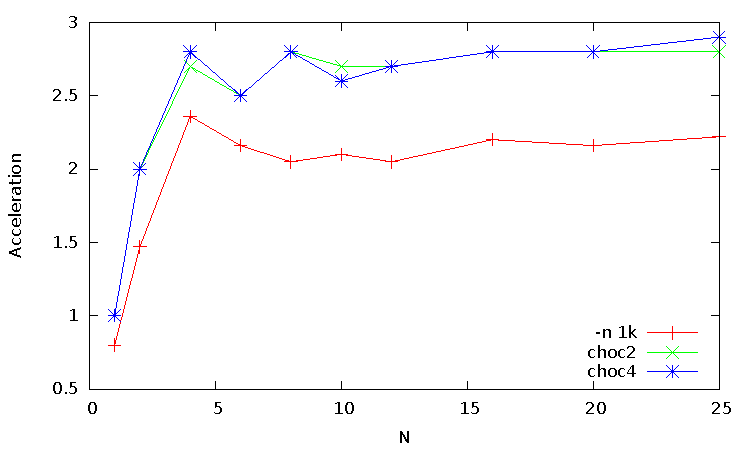
\includegraphics{Courbe/Difference_domain_initial.pdf}\\

\paragraph{}
Avec les domaines de initiaux $choc2$ et $choc4$, l'accélération augmentes jusqu'à stagner. Alors que pour le domaine initial $-n 1k$ , l'accélération augmente, puis diminue jusqu'à stagner. La diminution de performance est du au fait qu'on crait trop de thread. Les threads ne sont plus rentable,la création d'un thread prend plus de temps que se que fait gagner le thread.

\subsection{Variations sur la politique de distribution d'indices}
Nous avons ensuite fait varier la politique de distribution d'indice,en modifiant la varaible d'environnement "OMP\_SCHEDULE". La distribution dite dynamique et static semble se valoir quand il y a peu de threads. Mais lors que le nombre de thread est important, la distribution dynamique semble meilleurs.\\

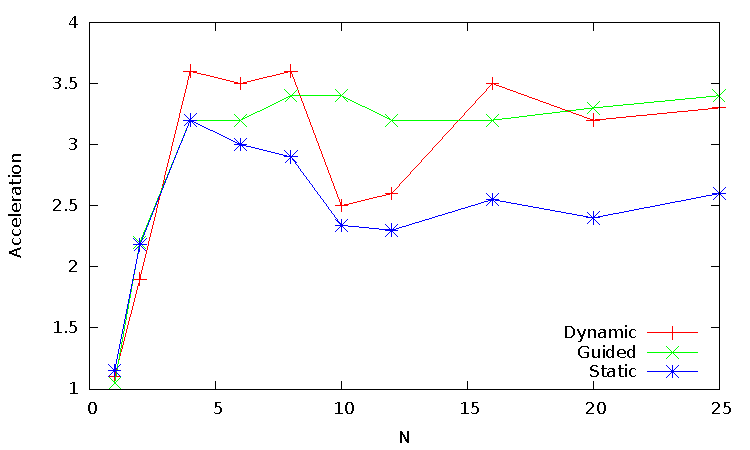
\includegraphics{Courbe/sch.pdf}
\subsection{Variations sur le placement des threads et de la mémoire}
\paragraph{}
Lorsqu'on utilise un seul coeur, les performances sont décroissantes. Ce qui est normal car on crait des threads sur un seul coeur et on perd du temps en interruption pour changer de thread sur le coeur. On remarque cependant qu'au bout d'un certain nombre de thread, nous récupérons une accélération de 1. Ceci doit être une optimisation automatique de l'ordinateur. 

\paragraph{}
Pour les autres cas, l'accélération augmente jusqu'a que le nombre de thread soit égale au nombre de coeur. Si le nombre de thread est supérieur au nombre de coeurs, l'accélération diminue à cause des pertes de temps pour changer les threads sur les coeurs.

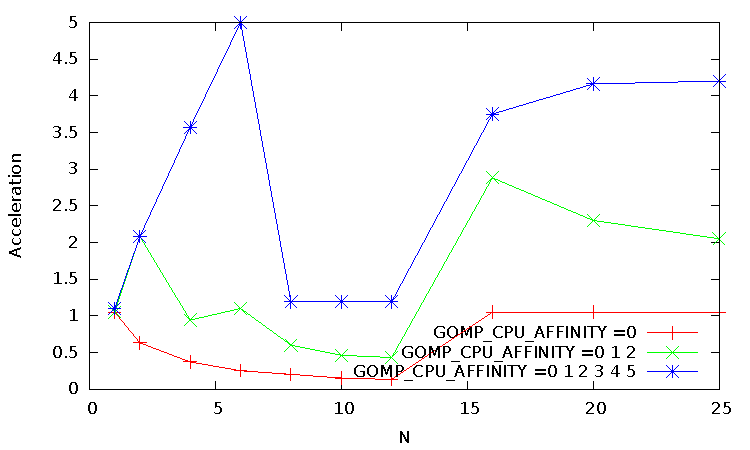
\includegraphics{Courbe/GOMP.pdf}
\subsection{Variation sur le type de machine}
On remarque que l'accélération varie selon la machine utilisé. La machine jolicoeur a de moins bonne performance que la machine de la salle 008.\\

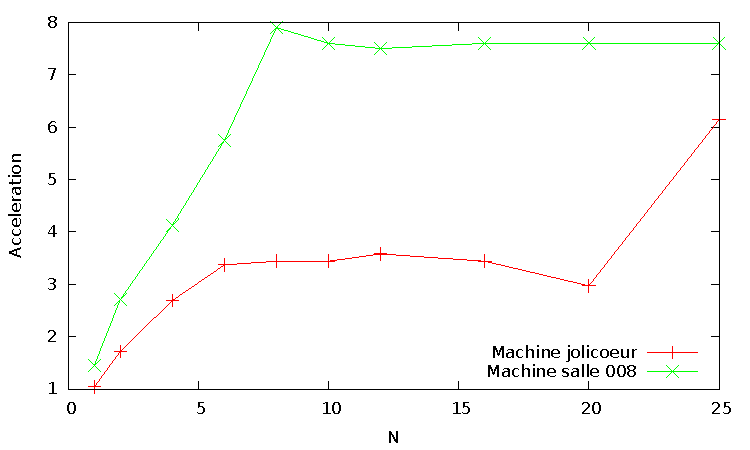
\includegraphics{Courbe/Difference_machine.pdf}

\section{Parallélisation avec \textbf{OpenCL}}
\subsection{Application de la gravité}


\begin{lstlisting}[style=CStyle]
// This kernel is executed with one thread per atom
__kernel
void gravity (__global calc_t * speed, calc_t gx, calc_t gy, calc_t gz,
	      unsigned natoms, unsigned offset)
{
    unsigned index = get_global_id (0);

    if(index < natoms){
     coord_t g;
     g.x =gx * -1;
     g.y = gy * -1;
     g.z = gz * -1;
     inc3coord(speed + index,g,offset);
    }
}
\end{lstlisting}

\subsection{Calcul des forces avec tri par boîtes}
\subsubsection{traitement de la somme prefixée}
\paragraph{}
Comme conseillé sur le sujet, nous avons fait une implémentation de la somme préfixée en dehors du projet. Ainsi, nous avons fait un module prescan, qui calcule len OpenCL , la somme préfixée d'un tableau d'entier. Le noyau OpenCL qui effectue le calcul est présenté ci après:
\vfill
\begin{lstlisting}[style=CStyle]
    __kernel  void prescan(__global const int *A,__global int *B,const  uint n)  
    {  
        __local int temp[SIZE];  // allocated on invocation  
        int thid = get_local_id(0);  
    	int offset = 1;  
	int last = 

    	temp[2*thid] = A[2*thid]; // load input into shared memory  
    	temp[2*thid+1] = A[2*thid+1];  
  	
    	for (int d = n>>1; d > 0; d >>= 1)                    // build sum in place up the tree  
    	{   
    	    barrier(CLK_LOCAL_MEM_FENCE);
       	    if (thid < d)  
       	    {  
	        int ai = offset*(2*thid+1)-1;  
		int bi = offset*(2*thid+2)-1;  
		temp[bi] += temp[ai];  		       
    	    }  
    	    offset *= 2;  
   
	    if (thid == 0) { temp[n - 1] = 0; } // clear the last element  
         }            
	 for (int d = 1; d < n; d *= 2) // traverse down tree & build scan  
    	 {  
     	       offset >>= 1;  
               barrier(CLK_LOCAL_MEM_FENCE);
               if (thid < d)                       
               {  
	       	  int ai = offset*(2*thid+1)-1;  
    	  	  int bi = offset*(2*thid+2)-1;  
		  float t = temp[ai];  
    	  	  temp[ai] = temp[bi];  
    	  	  temp[bi] += t;   
          	}  
    	 }  
     	 barrier(CLK_GLOBAL_MEM_FENCE);

	 B[2*thid-1] = temp[2*thid]; // write results to device memory  
	 B[2*thid] = temp[2*thid+1];  
	 barrier(CLK_GLOBAL_MEM_FENCE);	 
	 B[SIZE - 1] = temp[SIZE - 1] + A[SIZE - 1];

    }  
\end{lstlisting}
\paragraph{}
L'algorithme a été pris sur le site \url{http://http.developer.nvidia.com/GPUGems3/gpugems3_ch39.html} en CUDA et a été adapté et légèrement modifié en OpenCL. N'ayant pas pu intégrer cette fonctionnalité dans le projet, nous nous sommes permis de mettre le module dans notre code source. Le fichier README dit comment le mettre en marche. 

\end{document}
